\documentclass[final]{beamer}
\usepackage[size=custom,width=121.92,height=121.92,scale=1.17]{beamerposter}
% 121.92 cm = 48 in: the ISEF maximum side-to-side display width.
\usepackage[utf8]{inputenc}
\usepackage{amsmath,amssymb,booktabs,graphicx,tcolorbox}
\tcbuselibrary{skins}

\definecolor{myblue}{RGB}{18,52,102}
\definecolor{mymid}{RGB}{42,86,150}
\definecolor{mylight}{RGB}{226,234,246}
\definecolor{panelbg}{RGB}{238,243,251}
\definecolor{provedc}{RGB}{28,100,52}
\definecolor{openc}{RGB}{160,42,42}

\setbeamercolor{block title}{bg=myblue, fg=white}
\setbeamercolor{block body}{bg=mylight, fg=black}
\setbeamertemplate{navigation symbols}{}
\setbeamertemplate{itemize items}[circle]
\setbeamerfont{block title}{size=\Large,series=\bfseries}
\setbeamerfont{block body}{size=\normalsize}
\setlength{\parskip}{5pt}

% a captioned figure panel, as in the methodology grid
\newcommand{\panel}[3]{%
  \begin{tcolorbox}[colback=panelbg,colframe=mymid,boxrule=0.9pt,
      arc=2pt,left=3pt,right=3pt,top=3pt,bottom=3pt,
      fontupper=\footnotesize]
    \centering
    {\color{myblue}\bfseries\footnotesize #1}\\[3pt]
    \includegraphics[width=#3\linewidth]{#2}
  \end{tcolorbox}}

\newcommand{\keybox}[1]{%
  \begin{tcolorbox}[colback=white,colframe=openc,boxrule=1.1pt,arc=2pt,
      left=5pt,right=5pt,top=4pt,bottom=4pt]
    #1
  \end{tcolorbox}}

\begin{document}
\begin{frame}[t]

%% ============================ HEADER ============================
\begin{beamercolorbox}[wd=\paperwidth,sep=14pt]{block title}
\begin{columns}[c]
  \begin{column}{0.17\textwidth}\centering
    {\footnotesize\color{white} Beal Bank Dallas Regional\\ Science and
     Engineering Fair\\[4pt] Mathematics}
  \end{column}
  \begin{column}{0.64\textwidth}\centering
    {\Huge\bfseries MAXIMUM NULLITY OF CYCLIC COVERS OF GRAPHS\par}
    \vspace{6pt}
    {\Large\itshape A monodromy ceiling, cyclotomic matrix certificates, and the
     first exact zero forcing numbers $Z(P(n,k))$ for $k\ge4$\par}
    \vspace{10pt}
    {\large Aryan Padarthi\par}
  \end{column}
  \begin{column}{0.17\textwidth}\centering
    {\footnotesize\color{white} Category: Mathematics\\[4pt]
     All code and certificates\\ are open and reproducible\\[4pt]
     Every claim is labelled\\ proved / computed / open}
  \end{column}
\end{columns}
\end{beamercolorbox}

\vspace{12pt}

\begin{columns}[t]

%% ======================= COLUMN 1 =======================
\begin{column}{0.265\textwidth}

\begin{block}{VISUAL ABSTRACT}
\centering
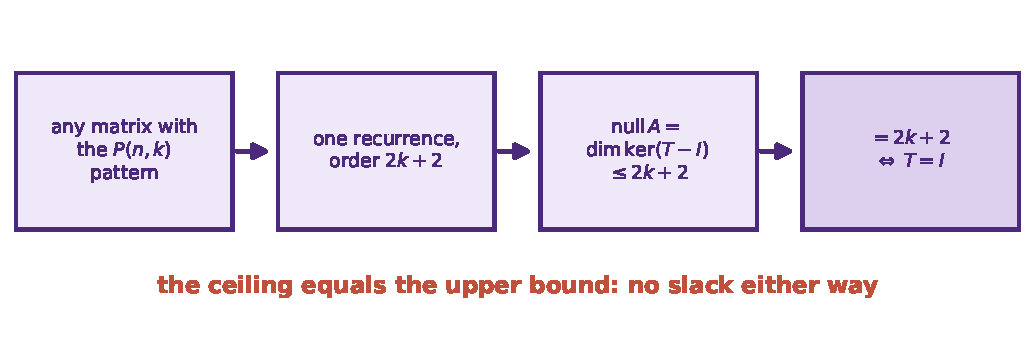
\includegraphics[width=\linewidth]{figures/fig_chain.pdf}\\[6pt]
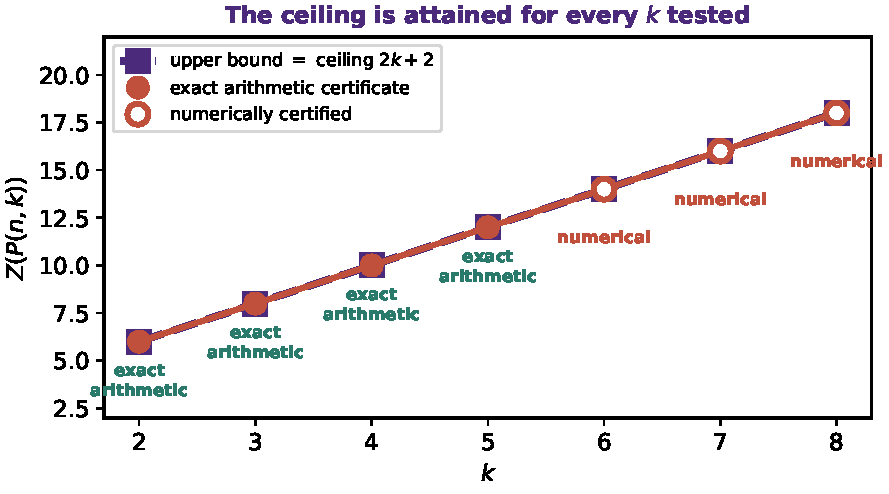
\includegraphics[width=\linewidth]{figures/fig_status.pdf}
\vspace{2pt}
\raggedright\footnotesize
Any matrix carrying the graph's pattern collapses to one linear recurrence.
Its order is $2k+2$ --- the same number as the best known upper bound --- so the
whole matrix method has a ceiling that exactly meets the target. This work
reaches that ceiling for $k=4$ and $k=5$.
\end{block}

\begin{block}{INTRODUCTION}
\textbf{The forcing rule.} Colour some vertices of a graph. If a coloured
vertex has exactly one uncoloured neighbour, that neighbour becomes coloured.
Repeat. $Z(G)$ is the size of the smallest starting set that eventually
colours everything.

\textbf{Why it matters.} $Z(G)$ bounds the \emph{maximum nullity} $M(G)$: the
largest null space of a symmetric matrix carrying the graph's pattern. The
parameter arose independently in quantum control and in power-network sensor
placement.

\textbf{The family.} $P(n,k)$: outer $n$-cycle $u_iu_{i+1}$, inner edges
$v_iv_{i+k}$, spokes $u_iv_i$. Cubic on $2n$ vertices, rotation
$\rho: i\mapsto i+1$.

\textbf{The general object.} $P(n,k)$ is a \emph{cyclic cover}: a base graph
$B$ with edge voltages in $\mathbb Z_n$ lifts to $V(B)\times\mathbb Z_n$. Two
vertices, loops of voltage $1$ and $k$, a spoke of voltage $0$ --- that is
$P(n,k)$. Everything below is really about covers.
\end{block}

\begin{block}{PROBLEM FRAMING}
Exact values of $Z(P(n,k))$ were known only for $k=2$ and $k=3$. A
\textbf{July 2026} correction note (arXiv:2607.19412) exists because a
published 2020 theorem is \emph{false}: it claimed $Z(P(n,3))=8$ for $n\ge12$,
but $Z(P(12,3))=7$ --- the case analysis never tested $7$-vertex sets. That note
closes with:
\vspace{4pt}
\keybox{\itshape ``Determining $Z(P(n,k))$ for general $k$ --- the stabilization
threshold and a rigorous lower bound for $k\ge4$ --- remains open.''}
\vspace{4pt}

\textbf{The asymmetry.} Upper bounds are easy --- exhibit one forcing set. Lower
bounds must rule out \emph{every} smaller set.
\end{block}

\begin{block}{RESEARCH OBJECTIVES}
\begin{enumerate}\setlength{\itemsep}{4pt}
\item Find the exact ceiling of the matrix-certificate method here.
\item Decide whether it can be attained, and construct certificates that do.
\item Make every certificate checkable in \textbf{exact arithmetic}.
\item Report which $k$ and $n$ are settled, and which are not.
\end{enumerate}
\end{block}

\begin{block}{WHY STANDARD METHODS FAIL}
A set is forcing iff it meets every \emph{fort}. Three standard consequences
all fail here, and all degrade as $k$ grows:
\begin{itemize}\setlength{\itemsep}{3pt}
\item \textbf{Disjoint forts:} at most \emph{two} exist in any case tested.
\item \textbf{Fort LP:} integrality gap $\approx2$ ($\mathrm{LP}=3.21$ against
      $Z=10$ for $P(18,4)$) --- which also explains why fort-based solvers
      scale poorly here.
\item \textbf{Spectral:} Hoffman-type bound gives $1.2$--$2.9$ against true $Z$
      of $6$--$12$.
\end{itemize}
Insufficient \emph{in principle}, not merely in practice --- which is what
motivated changing the category of argument.
\end{block}

\end{column}

%% ======================= COLUMN 2 =======================
\begin{column}{0.435\textwidth}

\begin{block}{MATHEMATICAL METHODOLOGY}

\begin{columns}[t]
\begin{column}{0.49\textwidth}
\panel{1. The colour change rule and the rotation bootstrap}{figures/fig_forcing.pdf}{1.0}
\end{column}
\begin{column}{0.49\textwidth}
\panel{2. Support of the reduced recurrence: nine terms, order $2k+2$}{figures/fig_recurrence.pdf}{1.0}
\end{column}
\end{columns}

\vspace{6pt}
\textbf{Step 1 --- Reduction.} Every spoke weight $c_i$ is nonzero, so the kernel
equation at $u_i$ solves for $y_i=-(b'_{i-1}x_{i-1}+a_ix_i+b_ix_{i+1})/c_i$.
Substituting into the equation at $v_i$ leaves \emph{one scalar recurrence} in
$x$, supported on nine indices with both end coefficients nonzero.

\keybox{\textbf{Theorem 1 (Reduction).} For every matrix $A$ whose off-diagonal
support is exactly $E(P(n,k))$ --- symmetric \emph{or not} ---
\[
  \operatorname{null}A=\dim\ker(T-I)\ \le\ 2k+2 ,
\]
$T$ the monodromy of that order-$(2k+2)$ recurrence, with equality iff $T=I$.
The order $2k+2$ is exactly the size of the forcing set the rotation bootstrap
produces: \textbf{the ceiling of the method equals the upper bound it is trying
to match.}}

\vspace{6pt}
\textbf{Step 2 --- The symbol.} For $A$ invariant under $\rho$, the Fourier
blocks are $M_m=\left(\begin{smallmatrix}a+s_m&c\\ c&d+et_m\end{smallmatrix}\right)$
with $s_m=2\cos\frac{2\pi m}{n}$. Since $t=L_k(s)$ exactly, where $L_k$ is the
monic integer polynomial with $L_k(z+z^{-1})=z^k+z^{-k}$,
\[
  \operatorname{null}A=\#\{m: F(s_m)=0\},\qquad
  F(s)=(s+a)L_k(s)+\alpha s+\beta .
\]
$F$ is monic of degree $k+1$ but carries \textbf{exactly three free
parameters, for every $k$}.

\vspace{4pt}
\keybox{\textbf{The key idea.} Three roots can be prescribed and no more --- but
prescribing three \emph{determines the other $k-2$}, and those land on the grid
$\Gamma_n=\{2\cos(2\pi m/n)\}$ by themselves whenever arithmetic puts them
there. If $F$ has \textbf{rational coefficients} its roots form Galois orbits,
and the Galois orbit of $2\cos(2\pi m/n)$ stays inside $\Gamma_n$. One rational
$F$ places all $k+1$ roots at once.}

\vspace{6pt}
\panel{3. The mechanism: every root of the symbol lands on the grid}{figures/fig_symbol.pdf}{1.0}

\vspace{6pt}
\textbf{Step 3 --- Cyclotomic construction.} Let $\Psi_d$ be the minimal
polynomial of $2\cos(2\pi/d)$, degree $\varphi(d)/2$. Choose distinct $d$'s with
$\sum\deg\Psi_d=k+1$, put $F=\prod\Psi_d$, and impose the $k-2$ integer
membership conditions. Every root then lies in $\Gamma_n$ for \emph{every} $n$
divisible by $\operatorname{lcm}(D)$.
\end{block}

\begin{block}{RESULTS \& COMPUTATIONAL VALIDATION}
\begin{columns}[t]
\begin{column}{0.48\textwidth}
\panel{4. Certificate spectrum: $12$ exact zeros}{figures/fig_spectrum.pdf}{1.0}
\end{column}
\begin{column}{0.50\textwidth}
\footnotesize
\centering
\begin{tabular}{@{}clll@{}}
\toprule
$k$ & $D$ & $F$ & result \\
\midrule
2 & $\{3,10\}$   & $sL_2-1$ & $6=2k+2$\\
4 & $\{4,30\}$   & $\Psi_4\Psi_{30}$ & $10=2k+2$\\
4 & $\{5,14\}$   & $\Psi_5\Psi_{14}$ & $10=2k+2$\\
4 & $\{5,18\}$   & $\Psi_5\Psi_{18}$ & $10=2k+2$\\
5 & $\{3,6,24\}$ & $sL_5-1$ & $12=2k+2$\\
\bottomrule
\end{tabular}
\vspace{6pt}

\raggedright
All have $a,\alpha,c\in\mathbb Z$: each certificate is an \textbf{integer
matrix}, and its nullity is confirmed by \textbf{exact rational Gaussian
elimination}, not by floating point.
\end{column}
\end{columns}

\vspace{6pt}
\keybox{\textbf{Main result.} With $Z(P(n,k))\le 2k+2$ from the bootstrap and
the certificates above,
\[
\begin{array}{ll}
 Z(P(n,4))=M(P(n,4))=10 & \text{for every }n\text{ divisible by }60,\ 70\text{ or }90,\\[2pt]
 Z(P(n,5))=M(P(n,5))=12 & \text{for every }n\text{ divisible by }24 .
\end{array}
\]
These are the \textbf{first exact values of $Z(P(n,k))$ for $k\ge4$}, the range
the 2026 note records as open. Both rest on \textbf{integer} matrices whose
nullity is confirmed by exact rational elimination.}

\vspace{5pt}
\textbf{Beyond $k=5$.} For $k\ge6$ the rotation-invariant symbol provably
cannot reach the ceiling: the enumeration of rational symbols is \emph{finite
and complete} and returns nothing. Relaxing to period $d$, the map from weights
to the $k+1$ symbol coefficients has $\operatorname{rank}=\min(2d+1,k+1)$ in
every case computed ($3\le k\le13$, $1\le d\le7$, returning the known $3$ at
$d=1$). Most weights are gauge, so every symbol becomes reachable exactly when
$d\ge\lceil k/2\rceil$ --- not the $d\ge(k+2)/5$ a naive count suggests.
\keybox{Taking $d=\lceil k/2\rceil$, the ceiling is attained for
\textbf{every $k$ tested}:
\[
 Z(P(60,6))=Z(P(72,6))=\mathbf{14},\quad
 Z(P(96,7))=\mathbf{16},\quad Z(P(96,8))=\mathbf{18},
\]
the first exact values for $k\ge6$. The required period was predicted in
advance by the rank law; $d=3$ then failed for $k=7,8$ where $d=4$ succeeded.
All verified on the full $2n\times2n$ matrix: correct cubic pattern, every
required entry $0.11$--$0.36$ of scale, and a spectral separation of eleven to
thirteen orders. \emph{Numerically certified; exact arithmetic pending.}}

\vspace{6pt}
\textbf{The $k=5$ certificate is the plain adjacency matrix:} $a=d=0$, $c=1$,
$sL_5-1=\Psi_6\Psi_3\Psi_{24}$. Its nullity we classify \emph{completely}: with
$P_k(z)=z^{2k+2}+z^{2k}-z^{k+1}+z^2+1$,
\[
 \operatorname{null}(\mathrm{Adj}\,P(n,k))=\!\!\sum_{\Phi_d\mid P_k,\ d\mid n}\!\!\varphi(d),
\]
a Conway--Jones phenomenon (rational relations among cosines of rational
angles). So $\mathrm{Adj}\,P(n,k)$ is \textbf{never} singular for $k=3,6,9$,
and attains the full ceiling only at $k=2$ and $k=5$. Checked against a direct
count for $k=2,5,8$ at every $13\le n<200$.
\end{block}

\end{column}

%% ======================= COLUMN 3 =======================
\begin{column}{0.265\textwidth}

\begin{block}{VERIFICATION \& CERTIFICATION}
No result here rests on floating point.

\textbf{Structural theorem:} $189$ random matrices over $63$ pairs $(n,k)$, plus
$60$ more for the determinant formula and product form. All pass.

\textbf{Cyclotomic certificates:} integer matrices; nullity by exact rational
elimination.

\textbf{Irrational certificates:} verified in $\mathbb Q(\zeta_n)$, with
$2\cos(2\pi m/n)$ as $x^m+x^{n-m}$ mod $\Phi_n(x)$ --- membership, reality, and
$c^2\ne0$ all decided exactly.

\textbf{Engine validation:} the exhaustive $Z$ solver reproduced \emph{every}
published value first, including the corrected $Z(P(12,3))=7$.

\vspace{4pt}
\keybox{\textbf{Two numerical traps, both caught by the ceiling.} A loose
tolerance reported nullity $7$ for $k=2$; a badly scaled candidate reported
nullity $48$ at $(n,k)=(48,7)$. Both are impossible by Theorem 1. \emph{Working
rule: wrap every numerical search in a bound it cannot legally violate} --- that
bound is the only thing that tells you an answer is wrong when it looks right.}
\end{block}

\begin{block}{CONCLUSIONS}
\begin{enumerate}\setlength{\itemsep}{4pt}
\item The method has an \textbf{exact ceiling of $2k+2$}, coinciding with the
      best known upper bound: either it settles $Z$ completely or nothing does.
\item The ceiling is \textbf{attained}, by rational symbols whose Galois orbits
      fall on the Fourier grid.
\item {\color{provedc}\bfseries Proved:} $Z(P(n,4))=10$ for $60,70,90\mid n$;
      $Z(P(n,5))=12$ for $24\mid n$; $Z(P(n,3))=8$ at $n=40,60,80,120$;
      $Z(P(n,2))=6$ for $9\le n\le130$, $n\ne10$.
\item {\color{openc}\bfseries Corrected (my own):} the claim that this
      construction ``never exceeds $6$'' was wrong, and the elaborate
      period-two machinery built to escape that cap was unnecessary.
\end{enumerate}
\end{block}

\begin{block}{FUTURE WORK}
\textbf{Honest limits.} The $k\ge6$ certificates are numerical, not exact ---
a weaker standard than $k=4,5$. The rank law is verified over a range, not
proved. At $n=48,54$, where the root set has no slack, every solution collapses
a spoke; we observe this rather than prove it. And exact certification via
\emph{rational} targets is closed: all eight Galois-closed root sets at $n=72$
hit the symbol to $10^{-15}$ with nullity $14$ and all eight degenerate.

\textbf{Next.} (i) Exact certification for $k\ge6$ by interval Newton --- the
ceiling theorem makes this tractable, since certifying the \emph{equation}
exactly gives the nullity as a discrete consequence; (ii) proving the rank law;
(iii) a construction valid for every $n$, not one $n$ at a time, which the
ceiling theorem would turn into a complete solution.
\end{block}

\begin{block}{KEY REFERENCES}
\footnotesize
[1] S. Rashidi, N. Shajareh Poursalavati, M. Tavakkoli, \emph{Computing the
zero forcing number for generalized Petersen graphs}, J. Algebra Combin.
Discrete Struct. Appl. \textbf{7}(2) (2020) 183--193.

[2] A. Krishnan, \emph{A correction to the zero forcing number of the
generalized Petersen graphs $P(n,3)$}, arXiv:2607.19412 (2026).

[3] AIM Minimum Rank Special Graphs Work Group, \emph{Zero forcing sets and the
minimum rank of graphs}, Linear Algebra Appl. \textbf{428} (2008) 1628--1648.
\end{block}

\end{column}
\end{columns}
\end{frame}
\end{document}
